% !Mode:: "TeX:UTF-8"
\documentclass[UTF8,a4paper]{ctexart}
\usepackage{geometry}
\usepackage{graphicx}
\usepackage{listings}
\usepackage{xcolor}
\usepackage{cite}

\definecolor{white-gray}{gray}{0.85}

\geometry{left=2.5cm,right=2.5cm,top=2.5cm,bottom=2.5cm}

\begin{document}
\title{summary}
\date{\vspace{-5ex}}
\author{student}
\maketitle
\thispagestyle{empty}
\newpage

\tableofcontents
\setcounter{page}{0}
\thispagestyle{empty}
\newpage

\section{研究背景及意义}

\section{研究目标及内容}

\section{相关技术综述}
\subsection{容器技术}
\subsubsection{容器技术简介}
容器是一种操作系统层的虚拟化运行环境, 该技术使得在同一个 Linux 宿主机上可以运行多个相互隔离的 Linux 系统容器. 容器技术的实现依赖于 Linux 内核所提供的 cgroups 和 namespaces 这两个功能模块, 前者可以在无虚拟机情况下提供进程对 CPU、内存、I/O 网络资源的访问限制和优先级控制, 而后者则可以完全隔离应用进程所看到的底层运行环境, 包括进程树、网络、用户ID和文件系统.

起初, 为了应对高性能计算集群中所遇到的困难\cite{Biderman2006}, Linux 内核xx版本中引入了称为 kernel namespaces 的特性. 基于该特性, 系统调用 clone() 可以创建出父进程全局 namespaces 的隔离实例. Linux 系统完整的实现了文件系统、进程号、网络、用户、进程间通讯和主机名的 namespaces. 例如, 每个文件系统都有自己独立的根目录和挂载表, 这有点类似于系统调用 chroot() 但是更为强大.

Namespaces 有多种不同的使用情景, 但最为常见的是创建对外界既不可知也无法访问的隔离容器. 运行在容器内的进程即使和其他 namespaces 中的进程共享底层内核, 也犹如运行在普通独立的 Linux 系统中. 此外, 容器也是可以层级嵌套的[], 但目前嵌套能力尚未完全探究清楚. 与运行整个操作系统的虚拟机不同, 容器最少只包含一个独立进程. 像完整操作系统一样运行 init, inetd, sshd, syslogd, cron 等进程的容器称为系统容器 (system container), 而运行其他应用的称为应用容器 (application container). 这两种的容器在适用于不同的场景. 例如, 应用容器会比系统容器和虚拟机消耗更少的 RAM, 因为它不需要其他额外的管理操作, 而这些应用容器通常没有独立的 IP 地址, 这在 IP 资源紧张的情况下相较于虚拟机而言是一大优势.

在完整隔离性非必要的情况下, 容器之间的资源共享也能简单实现. 例如, 由于 Linux 系统只 VFS 层[]的存在, 挂载绑定可以让目录挂载到多个容器内, 即使容器内目录位置不同. 此外, 容器与容器之间或容器与宿主机之间的通讯如普通 Linux IPC 一般高效.

Linux 中的 control groups(cgroups) 子系统用于将进程分组并管理它们的资源消耗. 它可以有效地限制容器的内存和 CPU 的使用量, 通过更改容器对应的 cgroups 限制便可以控制容器的资源消耗量. 此外, cgroups 也为容器中的进程提供了可靠的终止方式. 这是因为容器化的 Linux 系统中只有一个内核, 该内核具备全局视角, 并且控制着全局的资源分配与调度.

容器资源管理方面一个悬而未决的问题就是容器内的进程并不知道其资源受限\cite{Kung2014}. 例如, 一个进程可以查看到系统中的所有 CPU, 但却实际上只能使用部分, 内存上亦是如此. 若一个应用运行在资源受限的容器内, 当其根据整个系统资源自动调节自身可用资源时, 会造成过分配(over-allocate)的问题.

目前, 比较著名的 Linux 容器管理工具有 LXC\cite{LXCweb}, systemd-nspawn\cite{Systemd2012}, lmctfy\cite{lmctfy}, Warden\cite{Warden} 和 Docker\cite{WhatisDocker}. 有人将 Linux 容器与 LXC 混为一谈, 事实上这是一个误区, LXC 是不过众多具体的 Linux 容器管理工具之一.

\subsubsection{容器和虚拟机的比较}
在云计算环境中, 由于不同的工作负载 (workload) 往往是共享运行节点的, 隔离与资源控制便成了最为关键的两个问题. 隔离是指在同一个系统中, 一个工作负载的执行不能影响同节点下其他工作负载的执行. 资源控制是指系统能够约束每个工作负载只能访问和使用特定量的资源.

在传统的云平台上, 虚拟机实现隔离和资源控制的方式简单而有效, 因为每个工作负载都可以在其独占的虚拟机内运行, 并且将该工作负载的资源约束转变成该虚拟机的约束, 然而这会带来一定的额外资源开销.

虚拟机是这么玩的...半虚拟化和全虚拟化

与其在虚拟硬件上运行整个操作系统, 基于容器的虚拟化技术通过修改现有的宿主机系统提供额外的隔离性, 该过程通常涉及为每个进程添加一个容器 ID 属性, 并且增加对系统调用的访问控制检查, 因而容器可以视为用户 (user) 和用户组 (group) 许可系统外的另一种层次上的访问控制. 事实上, Linux 内核采用了更为复杂的设计与实现, 下文将做简要描述.

图表总结????

\subsubsection{基于容器和基于VM的云平台的比较}

\subsubsection{Docker}
Docker 的官方宣传语是 "Build, Ship and Run Any App, Anywhere".
Docker是Docker公司的一个开源项目, 它提供了以一种系统化方式在可移植的容器内部署自动化部署Linux应用. 事实上, Docker分别在Kernel和Application层的API对LXC进行扩展, 这些API协作使得进程运行的同时保持相互隔离的状态:CPU、内存、I/O和网络等. Docker容器可以通过基本镜像创建, 一个Docker镜像可以只包含系统级的基本组件, 也可以特定应用启动所需的复杂预置依赖栈. 当Docker创建镜像时, 每次操作都会在已有的层级结构上构造新的依赖层. 下图表现了基于虚拟机的应用部署和基于容器的应用部署之间的区别. 从 Docker 0.9 版本开始, 放弃LXC而采用自家的libcontainer.
\begin{figure}[htb]
     \centering
     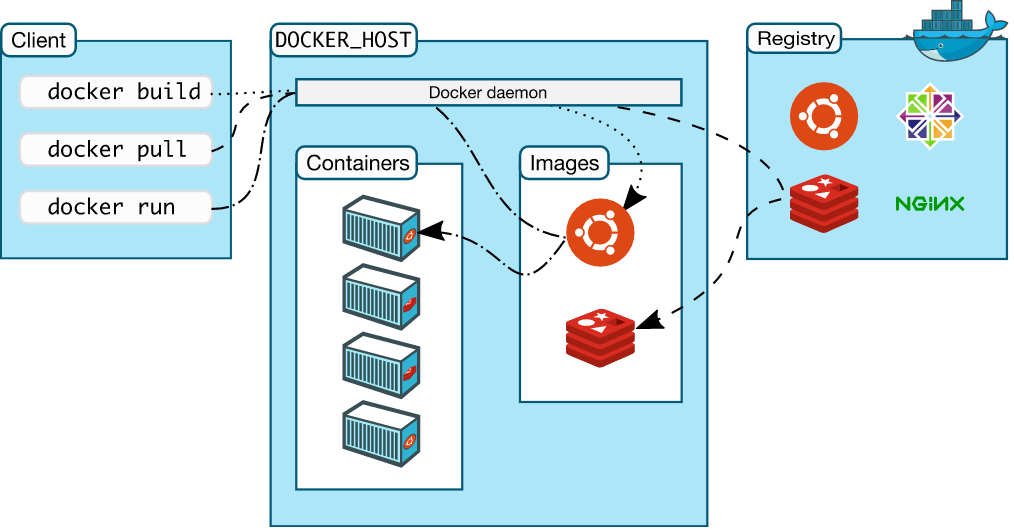
\includegraphics[width=.9\textwidth]{diagram/docker_arch.png}
     \caption{Docker 平台架构图}
     \label{docker_arch}
\end{figure}

\subsection{基于VM和物理机的集群管理系统}
\subsubsection{Borg}
Google公司最近公布了他们基础设施系统王冠上的宝石之一: Borg\cite{Borg2015}, 集群调度系统. Borg 系统主要提供了如下特点:
\begin{itemize}
    \item 隐藏了资源管理和失败处理的细节, 因此用户可以专注于应用部署.
    \item 提供高可用和高可靠的操作.
    \item 可以有效地在包含数以万计的机器集群上运行工作负载.
\end{itemize}

\subsubsection{Mesos}
Mesos\cite{Mesos2011} 是Apache下的开源分布式管理框架, 素有分布式系统内核之美誉.

要了解Mesos, 首先要了解 Mesos 存在的意义. 如今, 大量相对廉价的服务器集群已经成为了云计算平台的物理机基础, 支撑着无数的网络服务和持续增长的数据集中型科学应用. 在大数据应用发展的驱使下, 研究人员和从业人员已经开发了多种用以简化集群下大数据运算的计算框架, 其中比较著名的有 MapReduce\cite{MapReduce2004}, Dryad\cite{Quincy2009}, MapReduce Online\cite{MROline2010}(支持流式计算), Pregel\cite{Pregel2010}(专注于图计算框架)等. 毫无疑问, 还会有更多全新的集群计算框架出现, 没有一种框架会适合于所有数据类型的应用. 为了针对特殊的应用类型选择最优的计算框架, 往往会有多种计算框架共存于同一集群之中. 依据计算框架复用集群可以极大地提高集群的利用率, 并有效地共享难以迁移的海量数据.

由于多种计算框架共存同一宿主集群, 它们之间的计算资源分配的问题无可避免. 由此催生的 Mesos 最初由加州大学伯克利分校的 AMPLab 实验室开发, 后作为开源项目交由Apache 基金会管理, 目前以为成...级项目. Mesos 主要用于解决依存于同一计算集群的多种计算框架之间计算资源共享问题, 为了支持如今计算框架的负载调度算法, Mesos 引入了称为资源邀约 (Resource Offer) 的分布式两级调度机制. 由 Mesos 决定为每个计算框架提供多少计算资源, 而框架作为资源接受者可以选择合适的资源分配作为自身的可使用资源. 具体算法会在下文中给出.

\subsubsection{Omega}
Omega\cite{Omega2013} 可以视作 Mesos 的继任者, Mesos 部分作者参与了 Omega 的设计与开发.

Omega 全新的基于共享状态的调度算法让资源邀约更近一步. 在原本的 Mesos 中, 所有的资源邀约都采用一种悲观的或者独占的方式. 在这种情况下, 一旦某份资源邀约已经提供给一个应用程序, 那么同一份资源邀约则不可以同时提供给其他应用程序, 直到邀约超时. 这大大地降低了资源的有效使用和程序的并发量. 但是在 Omega 中, 资源邀约都是乐观的. 这意味着同一份资源邀约可以提供给不同的应用程序, 每个应用程序也可以申请集群中所有的可用资源, 如果发生冲突则交由 Omega 仲裁解决.

\subsubsection{Yarn}
Yarn\cite{Yarn2013}, 是 Yet Another Resource Negotiator 的缩写, 意为 "另一种资源协调者".

\subsection{基于容器的集群管理系统}
\subsubsection{编排部署三剑客: Machine、Compose和Swarm}
租用 Infrastructure as a Service (IaaS) 上廉价的硬件资源当下已成为不少公司的选择, 为了在各个 IaaS 平台上都能简易的运行 Docker 平台, Docker 公司推出了 Machine\cite{Docker-machine} 工具用于帮助用户在不同提供商的云主机上创建和管理虚拟机, 并在其中安装 Docker. 目前支持的虚拟机引擎有 Virtual Box, VMware Fusion 和 Hyper-V, 涵盖了 Linux、OS X 和 Windows 三大主流平台.

如果单单是在本地建立包含 Docker 的虚拟机, 并不是很振奋人心的是. Machine 真正的魅力在于充分利用了开源社区的力量, 为每个 IaaS 平台开发了一套对应的驱动以对虚拟机内的容器进行一系列轻量级操作. 目前, Machine 所支持的 IaaS 平台已经超过10中, 其中包括三大主流服务 Amazon Web Services、Microsoft Azure 和 Google Compute Engine.

Docker 对于个人开发者而言, 简单而实用, 但是随着容器云 Container as a Service (CasS) 的发展, 因容器规模的急剧增加, 手动管理 Docker 容器的方式不再可行. 如何批量的创建、调度和管理成了制约以 Docker 为代表的容器技术构建大规模集群的重要障碍.

很长一段时间内, Fig 都是编排和部署 Docker 容器集群的唯一选择. 2014 年 7 月, Fig 被 Docker 公司收购并构成官方项目 Compose (即为 docker-compose)\cite{Docker-compse}. 当需要以容器构建服务集群时, 集群内包含的容器数目可能十分庞大, 而容器之间的联系和拓扑结构也可能十分复杂. 单一的 Dockerfile 重现一个容器, 而 Compose 则重现了容器的配置与所构成的集群. 这便是 Compose 存在的意义. 通过 Compose 文件定义容器之间的关联与组织方式, 可以简单地实现控制该容器集群的生命周期. 使用 Compose 通常分为如下三个步骤:
\begin{enumerate}
    \item 用 Dockerfile 定义程序运行时环境, 容器在任何环境中都能重现.
    \item 在 docker-compose.yml 中定义构成独立应用的服务, 这样在相对隔离的环境中定义的容器能以集群的方式相互协作.
    \item 以简单的 docker-compose up 命令启动服务集群.
\end{enumerate}

一个简单的 docker-compose.yml 文件如下, 定义了一个 redis 为数据库的 web 项目:
\begin{lstlisting}[backgroundcolor = \color{white-gray}, framexleftmargin = 1em]
web:
  build: .
  ports:
   - "5000:5000"
  volumes:
   - .:/code
  links:
   - redis
redis:
  image: redis
\end{lstlisting}

在容器集群中, 把调度粒度停留在单个容器上是非常没有效率的. 因此, 集群化管理是有效提高对 Docker 管理效率和利用率的方式. 同为 Docker 公司出品的 Swarm\cite{Docker-swarm} 旨在在更高的抽象层次上使用 Docker, 即为将多台 Docker 平台主机逻辑上抽象成一台单一主机. 由于 Swarm 使用了标准 Docker API, 任何能与 Docker 通讯的工具都可以使用 Swarm 透明地扩展到多主机情景.

由于 Swarm 管理了多台 Docker 主机, 当用户在主机资源池中创建容器时, 容器的调度问题在所难免. 目前, Swarm 提供了 filter 功能, 用于筛选符合条件的主机. 之后, Swarm 使用 strategy 策略在符合条件的候选主机中选择最优主机. 现阶段 Swarm 提供了 random 和 binpacking 两种策略, random 模式即为在候选主机中随机选择一台, 而 binpacking 模式则会权衡主机 CPU 和内存使用率后选择消耗最小的主机.

像其他 Docker 项目一样, Swarm 也遵循 "swap, plug and play" 三原则.

\subsubsection{编排基石: Fleet}
偏向底层的容器编排部署工具 Fleet\cite{CoreOS-fleet} 出自大名鼎鼎的 CoreOS 团队之手, 它的官方定位是 "a distributed init system". 从设计上看, Fleet 和 Swarm 有异曲同工之妙, 若将 Swarm 理解成集群上 Docker daemon 的统一抽象, 那么 Fleet 则是提供了多个 systemd 的统一抽象. 单纯就 Fleet 而言, 它面向 systemd 单元, 而并不是一个容器管理或者编排工具, 它仅提供了集群中 systemd 单元的最为基本的调度功能, 从而构成了上层容器调度编排的基石, 尤其在容器间的亲密关系、Placement 规则、调度策略、高可用保障等重点条目上给出了合理的解决方案.

\subsubsection{集大成者: Kubernetes}

\subsection{Kubernetes}
\subsubsection{Kubernetes简介}
Kubernetes 是一种在集群中能够跨多服务器, 用于管理容器化应用的开源系统, 其设计目的在于简化容器化或者基于微服务的应用部署过程的同时保持部署功能的完整性和强大性.

Kubernetes 为应用的部署、调度、更新、维护和缩放 (scaling) 都提供了相应的机制. 其一个关键的特点在于它能够动态的管理容器以确保容器的状态能够持续地符合用户的意图. 实际的用户能够简单的启动一个微服务, 而让Kubernetes 的调度器为该服务找到合适的运行节点. We want to. . .

Kubernetes 目前仅支持 Docker 和 Rocket 这两种容器, 将来也会支持其他的容器镜像格式和容器运行时.

尽管 Kubernetes 当前专注于持续运行且无状态的应用(例如  web服务器内存对象缓存)和 "Cloud Native" 有状态应用(例如 NoSQL 数据存储), 在不久的将来也会支持在实际的生产环境中常见的工作任务类型, 例如批处理、流处理和传统数据库.

在 Kubernetes 中, 所有的容器都在 Pod 内运行. 一个 Pod 中可以仅存在单个容器也可以存在多个相互协作的容器. 在后一种情况中, 该Pod中的容器将被调度到同一个节点上, 并且相互之间共享资源. 此外, 一个Pod既可以不包含数据卷, 也可以包含多个数据卷, 这些数据卷既可以是某个容器私有的也可以是多个容器共享的. Kubernetes会为用户创建的每个Pod都寻找一个健康且拥有足够资源的节点, 并且在该节点上启动相应的容器. 若该Pod启动失败, 该节点上的节点代理Kubelet会自动的尝试重新启动. 但若该Pod或者该节点失效了, Kubelet并不会自动迁移或者重启该Pod, 除非用户定义了Replication Controller以确保Kubernetes中有指定数目的特定Pod实例在运行.

用户可以自己创建并管理Pod, 但Kubernetes彻底地简化了系统管理过程, 因为Kubernetes允许用户委派两种常见的Pod活动:一是基于相同的Pod配置部署多个Pod副本, 二是当Pod或所在节点失效时, 重新创建替代的Pod. 管理这些行为的Kubernetes API称为Replication Controller. 它以模板的方式定义Pod, 然后有系统实例化用户指定数量的Pod. 这些重复的Pod进而构成一整个应用、一个微服务或者多层应用中的某一层. 一旦Pod被创建, 系统将会持续的监控它们本身和所在节点的运行状况;当Pod 由于软件问题或节点故障失效时, Replication Controller将会在动的在一个健康的节点上重新一个全新的Pod, 以将该Pod的个数维持在稳定的数目.

Label. . .

Kubernetes支持一种独特的网络模型, 它鼓励扁平的地址空间管理方式, 并且让用户自己选择合适方便使用的端口而不是动态分配, 最终每个Pod都会分配到一个独立的IP地址.

现代的网络应用通常以层次化微服务的方式组建, 例如, 在一个分布网站中, 一组前端与分布式的写内存的键值存储交互, 而该键值存储进而与冗余的写磁盘存储服务交互. 为了简化该网络模型, Kubernetes提供了称为service的服务抽象, service为所对应的一组构成微服务的动态Pod提供了一个稳定的IP地址和DNS名. 所选Pod集合以标签选择器的方式定义, 所以可以指向任何Pod集. 当一个容器在Kubernetes中运行时, 运行于宿主节点称为kube proxy的本地代理将以转发的方式使容器连接到该IP地址, 后端以轮询策略确保负载均衡. 此外, kube proxy也负责追踪动态的Pod集合, 当新创建的Pod取态失效Pod时, kube proxy会选取新建Pod作为后端, 所以服务的IP地址永远不会变.

Kubernetes中的每一种资源, 例如Pod, 都会以URI标识并用于独一无二的UID.

\subsubsection{Kubernetes架构}
\begin{figure}[htb]
     \centering
     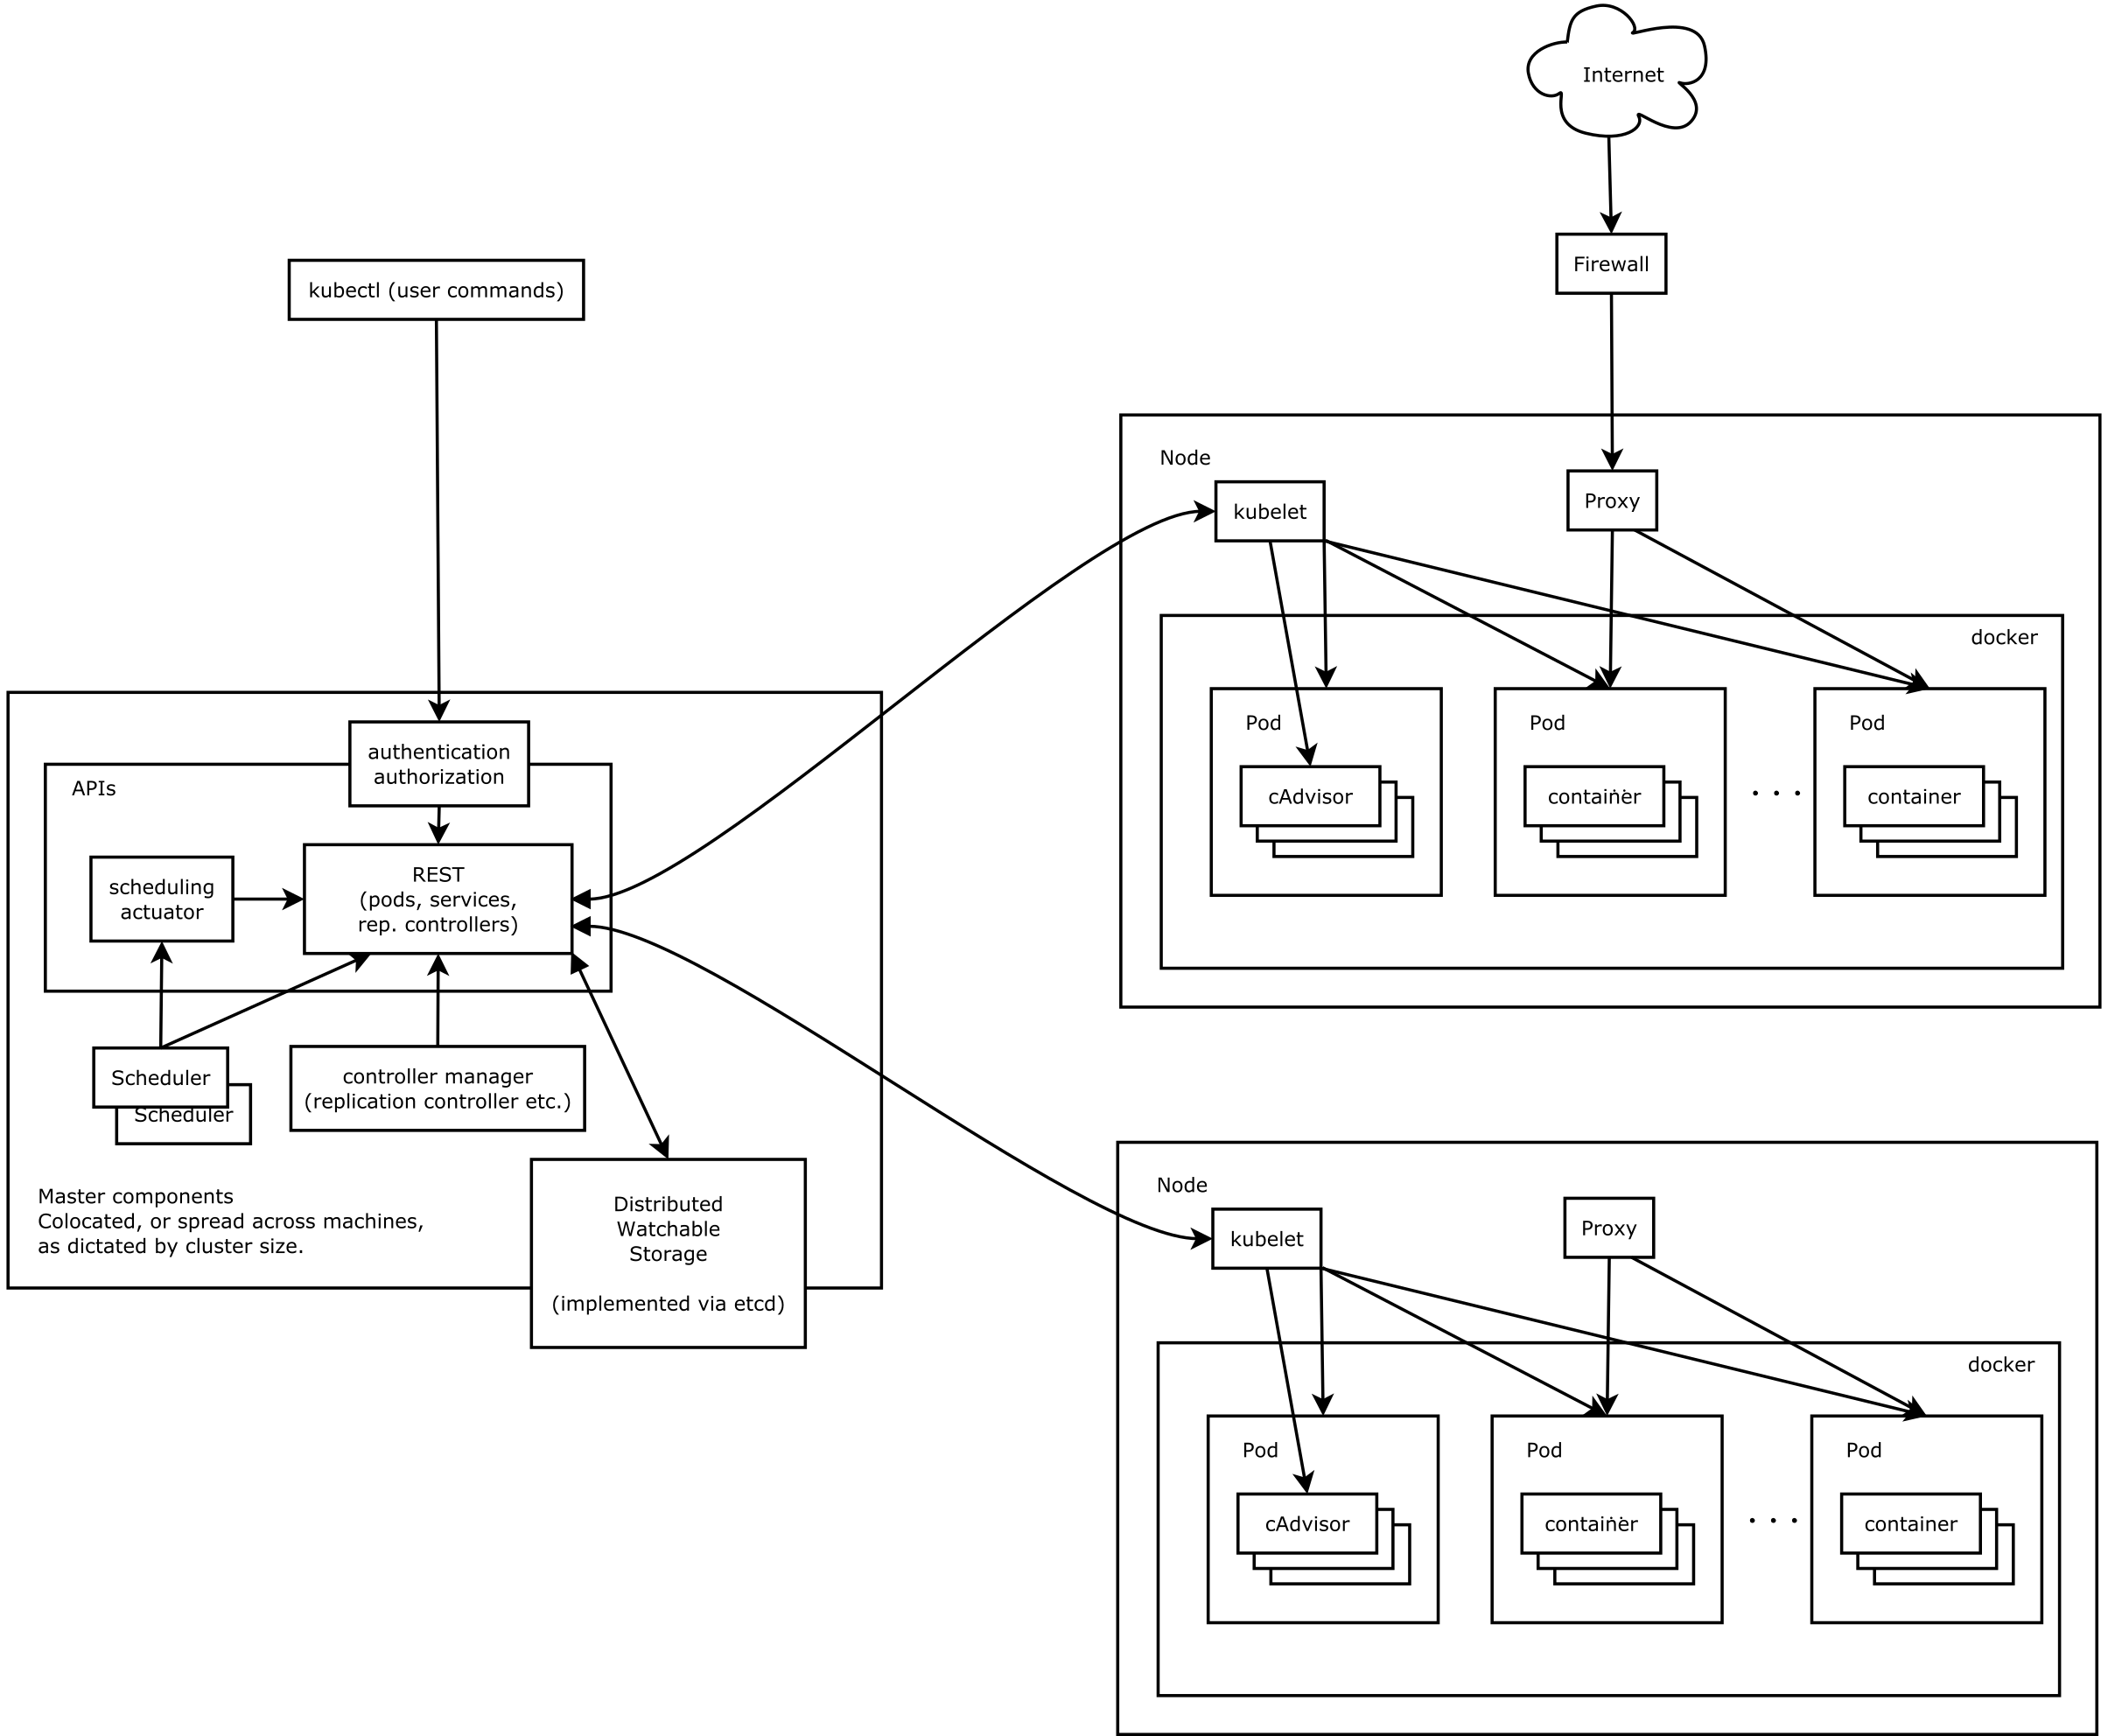
\includegraphics[width=.9\textwidth]{diagram/k8s_arch.png}
     \caption{Kubernetes 系统架构图}
     \label{k8s_arch}
\end{figure}

\subsubsection{从Borg到Kubernetes}
Kubernetes是由Google公司内部早已高度成熟的Borg系统演进而来, Borg系统是Google公司集群管理系统, 该系统可以同时运行数以万计的任务, 并且它可以跨集群运行, 每个集群都支持一万台机器. 2015年的Eurosys国际会议上, Google公司公布了从Borg到Kubernetes发展的相关细节.
\begin{figure}[htb]
     \centering
     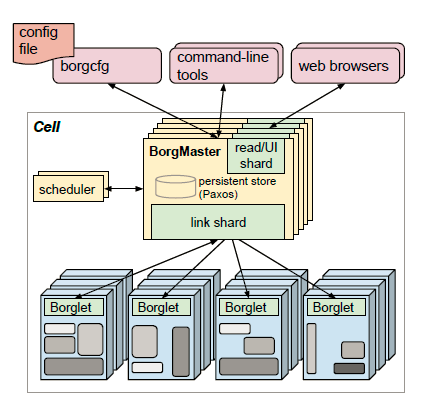
\includegraphics[width=.6\textwidth]{diagram/borg_arch.png}
     \caption{Borg 系统架构图}
     \label{borg_arch}
\end{figure}
比较 Kubernetes 和 Borg 的系统架构图, 就知道他们之间存在诸多共性, 其实, Kubernetes最重要的贡献者中不少曾都参与Borg系统的开发. 设计之初, Kubernetes以成熟的Borg系统为蓝本, 保持Borg在应用准入、调度、启动、重启和监控等核心功能的同时, 强调了自身的模块性和可理解性, 在集群管理功能的全面性和复杂性上有所折中. Kubernetes将Borg系统中所运用的技术和经验以容器的角度重新定制, 下文从四个方面分析Kubernetes从Borg所沿袭并发展的理念.

首先, 是调度部署单元. 在Kubernetes中, 最基本的资源和任务的调度单元是Pod, 它用来定义包含一个或多个相关容器的容器组, 并通过ReplicationController来将同一个模块单元部署到指定数量的容器组中, 实现了每个容器组生命周期的自动化管理, 极大的简化了系统部署和管理的工作量和成本. 而在Borg系统中, 也有功能类似的调度单元, 称为Alloc, 是allocation的缩写, 它的官方定义是“a reserved set of resources on a machine in which one or more tasks can be run; the resources remain assigned whether or not they are used.”[], 即为资源分配与任务调度的基本单元. Kubernetes在每个容器只运行一个应用这种服务模式的基础上, 又拓展了多个进程可以运行于同一个节点上的功能. 由此可见, Pod既继承了Alloc的核心理念同时, 又结合当前的实际予以创新.

其次, 是集群管理. 在Borg系统中, 细粒度的任务或机器构成了系统所管理的基本对象, 但是, Borg需要为整个系统中所运行的应用提供集群层次的负载均衡功能和重命名服务. 这些集群层次的高效管理方法促成了Kubernetes中Service这一概念的诞生, Service也直接构成了Kubernetes系统中的基本操作单元, Service作为应用所提供真实服务的抽象, 对外表现为一个单一的访问接口, 这样, 在后端实际运行完全透明的情况下也可以正常使用它所提供的服务, 有利于后端的维护和扩展工作.

再者, 是调试技术. 由于 Borg 作为 Google 公司内部使用的分布式应用管理系统, 调试信息也会直接暴露给使用人员. 此外, 为了进一步方便调试, Borg 还提供了针对各种层次的调试工具和用户接口. 这样, 即使面对大量的日志数据时, 用户也可以针对自己所遇到的实际问题进行日志分析. 同样, Kubernetes 也为用户提供了相类似的调试工具, 如资源控制工具 cAdvisor 和基于 Elastic Search 的日志聚合工具, 它们有效的简化了用户调试工作, 极大的缩短了调试时间.

最后, 是关于主节点 Master 在整个分布式系统中的作用与地位. Borg 和 Kubernetes 整体都是 Master-Slave 架构, 在 Borg 中, Master 节点其实是一个运行于单元层上的控制器进程, 它保存着所有节点代理 Borglet 上的状态数据. 作为 Borg 系统的入口和核心, Master 提供了准入控制、任务提交等一系列服务. 而在 Kubernetes 中, 以此为基础, 提供了强大的请求处理和管理下层对象状态的 API Server.

由上可知, Borg 系统的成功孕育出了 Kubernetes 的卓越设计理念. 作为 Borg 系统的继承与发展, Kubernetes 也试图解决 Borg 系统中所存在的问题. 例如, 在 Borg 系统中, 任务 Task 唯一的成组机制是 Job 单元, 但对于 Task 中的部分 Job 或者 Job 中的部分服务. 在 Kubernetes 中, 则提供了 Label 机制以实现局部管理.

\subsection{分布式一致性存储}
\subsubsection{CAP原则}
在2000年 PODC 会议上, 加州大学伯克利分校的 Eric Brewer 教授在特邀演讲中提出了著名的 CAP原则\cite{CAP2000}, 是说在一个异步的网络中, 读写式存储操作实现不可能同时满足以下三个属性:
\begin{enumerate}
    \item Consistency, 及在所有节点上的读写操作都是原子的或线性一致的.
    \item Availability, 及对数据读写的请求最终都会完成.
    \item Partition tolerance, 及允许网络丢弃任何信息.
\end{enumerate}
\subsubsection{Etcd简介}
Etcd是CoreOS所开发和维护的一个分布式的、强一致性的键值存储服务, 该开源项目托管在 github 上, 它主要用于共享配置和服务发现, 主要有如下特点:
\begin{enumerate}
    \item 简单, 面向用户curl可读的API(HTTP+JSON);
    \item 安全, 可选的SSL客户端证书认证机制;
    \item 快捷, 支持每个实例每秒1000次写操作;
    \item 可靠, 使用Raft算法实现了分布式环境中的强一致性.
\end{enumerate}

Etcd的灵感源于Zookeeper和Doozer, 它作为Docker生态系统重要的成员, 同样也使用 Go 语言开发并实现了 Raft \cite{Raft2014}一致性算法, 以管理高可用性的冗余日志. 目前, etcd 已在其他公司产品的生产环境中得到了广泛的使用, 其中著名的有 CoreOS 公司的分布式 init 系统 fleet、VMware 所发起的开源 PaaS 平台 Cloud Foundary 以及 Google 公司的容器集群管理系统 Kubernetes.

\subsubsection{Etcd和Doozer、Zookeeper的比较}
与etcd类似, zookeeper是在分布式系统系统中集中化服务, 主要用于维护分布式配置信息、命名服务、提供分布式同步以及组服务. 该项目基于Zab协议以Java语言实现集群之间的信息一致性.

通常, zookeeper运行于包含3、5、7等奇数节点的集群上, zookeeper 客户端

在zookeeper中, 服务注册是在特定名空间下以临时节点(ephemeral node)实现的的. Ephemeral nodes only exist while the client is connected so typically a backend service registers itself, after startup, with its location information. 一旦该连接失败或断开, 该临时节点也不在存在.

而zookeeper中的服务发现是以罗列(list)并观测(watch)服务的名空间方式实现的. 当某服务变得无法获取或有新服务注册时, 客户端会获取到当前所有可用服务和通知(notification). 此外, 客户端需要自己处理负载均衡和失效备援(failover).

zookeeper的api难以准确的使用, 而且语言绑定稍有差池便会造成问题. 若开发中使用了基于JVM的语言, 工具Curator Service Discovery Extension 可以提供不少帮助.

由于zookeeper是一个CP系统, 当存在网络分区(partition)时, 即便系统的某些部分可以看似正常的工作, 事实上它们是不能够发现现有注册组件(registration)以及注册的. 尤其是当某网络分区内未达到最少节点数要求时, 读写操作都会返回错误.

Doozer是一个基于Paxos协议, 以Go语言实现的强一致性、分布式数据存储系统. 很不幸的是, 该项目发展数年之后陷入了停滞状态, 也难以确定该项目是否已在生产环境中得以运用.

同样, Doozer通常也是运行于包含3、5、7等奇数节点的集群上, 于Zookeeper相似, Clients use language specific bindings to access the cluster, 此外, 集成已经嵌入到客户端与服务之中.

由于Doozer没有任何零时节点的概念, Doozer中的服务注册并不像Zookeeper中的那样直观, 服务会在特定的路径下注册自身, 但当该服务无法获取时, 它也不会自动移除. 有几种方法解决该注册失效的问题, 其中一种是依赖时间戳与心跳机制维系所注册的服务.

Doozer中的服务发现与Zookeeper十分相似, 及列出某路径下的所有项(entry), 然后等在路径下的任何变化(翻译的好拗口). 若使用了时间戳与心跳机制, 一旦心跳间隔超时, 就该移除此服务项.

与Zookeeper一样, Doozer也是一种CP系统, 在网络分区下会和Zookeeper存在同样的问题.

表总结了Zookeeper、Doozer和Etcd之间的异同.
\begin{table}[!hbp]
    \centering
    \begin{tabular}{c|c|c|c|c|c}
    名称& 类型& AP/CP& 语言& 依赖& 集成方式 \\
    \hline
    Zookeeper& 通用型& CP&  Java& JVM& 客户端绑定 \\
    Doozer& 通用型& CP& Go& & 客户端绑定 \\
    Etcd& 通用型& 混合& Go& & 客户端绑定/HTTP \\
    \end{tabular}
    \caption{分布式一致性服务对比}
\end{table}

\subsection{分布式调度技术}

\begin{table}[!hbp]
    \centering
    \begin{tabular}{c|c|c|c|c}
    方法& 资源选择& 冲突处理& 分配粒度& 集群策略 \\
    \hline
    整体调度& 所有可用& 无(序列化)& 全局策略& 绝对优先级(抢占式) \\
    静态划分& 固定子集& 无(静态划分)& 每个划分独立策略& 调度器相关 \\
    两级调度& 动态子集& 悲观算法& 贮藏(Hoarding)& 绝对公平 \\
    共享状态& 所有可用& 乐观算法& 每个调度器独立策略& 自由竞争的优先级抢占 \\
    \end{tabular}
    \caption{集群调度算法对比}
    \label{schedulers_comparison}
\end{table}

\subsubsection{整体调度}
整体调度是分布式系统中最早使用的调度算法, 它不存在并行. 整体调度器作为调度算法代码的唯一运行实例, 对所有的工作负载使用单一的资源管理和调度系统. 这种调度系统广泛应用于高性能计算中. 也有一些高性能计算调度器通过引入权重因子计算策略的优先级的方式支持多策略调度, 例如 Maui\cite{Maui2001} 以及它的继承者 Moab, 以及 LSF平台\cite{Iqbal2005}.

整体调度中, 另一种支持多策略调度的方法是在调度器代码中实现多条策略路径, 从而达到为异构的工作负载使用不同调度算法的目的. 这种方式虽然思想简单, 但实现起来难度很大. 例如 Google 的 Borg 系统就采用了这种实现方式, 此外 Google 公司通过不断地优化算法和框架, 使该系统支持内部并发并使用多线程技术处理队首阻塞和扩展性.

虽然这种整体调度算法实用而高效, 但它所存在的问题也十分明显, 及在现有整体调度算法的框架下, 难以便捷地添加新的策略和特定的实现方式\cite{Omega2013}, 此外整体调度难于适应集群增长的情况.

缺点:单实例, 无并发, 单代码块实现所有逻辑

\subsubsection{静态分配调度}
大部分云计算调度系统, 例如大名鼎鼎的 Hadoop\cite{Hadoop2010} 和 Dryad 的 Quincy\cite{Quincy2009} 系统, 都假设它们对特定的计算资源集合拥有完整的控制权, 因为集群往往会被静态地划分成几个独立的部分并分配专属资源, 或者集群中单一的调度器会被分成几个部分以支持多种不同的调度行为\cite{Yanpei2012}. 这就导致了存储残片和次优使用率的问题.

\subsubsection{两级调度}
静态分配调度方式的缺陷就在于全局资源的静态分配, 一种显而易见的解决方案就是动态地决定各个调度器的资源分配情况. 通常由一个统一的资源协调者为多个相互独立的调度框架提供计算资源. 这种两级调度方式目前也被广泛使用, 最为著名的是上文提到的 Mesos 系统和 Hadoop-on-Demand(HOD)\cite{HOD2012} 系统.

在 Mesos 系统中, 集中式的资源管理器动态地划分集群并为每个子集群的调度框架分配计算资源. 所有的可用资源都会以资源邀约 (Resource Offer) 的形式分发给各个调度框架, 但为了避免冲突, 每次资源管理器只会将一份资源邀约提供给一种调度框架, 与此同时, 资源管理器试图以选择资源邀约的体量和顺序的方式达到绝对的资源分配均衡 (DRF)\cite{DRF2011}. 由于需要用加锁机制来确保每份资源邀约只能提供一种调度框架候选, 所以 Mesos 的并发控制是悲观的.

相较而言, Yarn 似乎也采用了一种两级调度方式, 每个 Job 的 Application Master 的资源请求都会发送给 Resource Master 中的一个全局调度器, 该调度器会依据应用指定约束为不同的节点分配资源. 但是每个 Application Master 仅仅提供 Job 管理服务, 并不提供调度, 所以 Yarn 其实是一种高效的整体调度架构.

\subsubsection{基于共享状态的调度}
多个可以访问全局资源的调度系统, 例如 Google 的 Omega.
而在基于共享状态的调度算法中, 没有统一的资源协调者, 所有的调度器都可以有权访问所有的资源, 并允许公平而自由的资源竞争, 当存在冲突时, 以乐观的并发控制协调冲突. 这便解决了两级调度中所存在的两个问题: 因悲观并发控制而造成的有限并行和每个调度器受限的资源可见性. 

目前, 采用基于共享状态的调度算法的系统主要为 Google 的 Omega. 由于 Omega 中没有统一的资源协调者, 所有的资源分配决策由各个调度器自行决定. 在集群中, 会保留一份称之为 \textit{cell state}\cite{HOD2012}的资源分配情况说明, 而每个调度器都拥有一份本地的私有副本, 该副本会频繁更新以用于资源分配决策. 每个调度器都可以看到 \textit{cell} 的完整状态, 并能够自由的竞争资源的使用权, 包括那些已经被其他调度器所获取的资源. 一旦有调度器决定占用资源, 它以原子操作的方式提交更新共享 \textit{cell} 状态的申请. 若同时有多个调度器提交申请并存在资源索取冲突, 最终只有一个能成功的获取资源的使用权: 从状态同步到申请尝试的过程是一个事务过程. 无论该事务是否成功, 调度器之后都会重新同步 \textit{cell} 的状态, 如果可能的话, 会再次提交资源申请. 

Omega 中所有的调度器以完全并行的方式运行, 而且不会等待其他调度器中的 Job, 所以不存在调度器内的队首阻塞问题. 为了防止竞争造成的饥饿问题, Omega 调度器通常采用增量事务算法 (incremental transactions) ... 当处理群组调度时, 调度器使用 all-or-nothing 的事务算法, 要么成功调度该 Job 的所有 tasks, 要么全部 tasks 放弃此次调度而等待下次重新调度. 这有利于解决资源贮藏 (hoarding) 的问题.

此外, 不同的 Omega 调度器可以实现不同的调度策略, 但所有的资源调度器都得对资源分配情况达成共识, 并以相同的标准评价 Job 的相对重要性. 在这种情况下, 两级调度中的集中化的资源协调者弱化为持续化数据存储和统一规则验证中心. 

\section{技术路线}
\section{课题创新}
\section{参考文献}
\begin{thebibliography}{0}
    \bibitem{Biderman2006}
    E. W. Biederman. Multiple instances of the global Linux namespaces. In Proceedings of the 2006 Ottawa Linux Symposium, 2006.

    \bibitem{Kung2014}
    Fabio Kung. Memory inside Linux containers. \\http://fabiokung.com/2014/03/13/memory-inside-linux-containers/, March 2014.

    \bibitem{LXCweb}
    Stphane Graber and others. LXC—Linux containers. https://linuxcontainers.org/.

    \bibitem{Systemd2012}
    Lennart Poettering and Kay Sievers and Thorsten Leemhuis. Control centre: The systemd Linux init system. http://www.h-online.com/open/features/Control-Centre-The-systemd-Linux-init-system-1565543.html, May 2012.

    \bibitem{lmctfy}
    Victor Marmol and others. Let me contain that for you: README. \\https://github.com/google/lmctfy/blob/master/README.md.

    \bibitem{Warden}
    Cloud Foundry Warden documentation. \\http://docs.cloudfoundry.org/concepts/architecture/warden.html.

    \bibitem{WhatisDocker}
    Solomon Hykes and others. What is Docker? https://www.docker.com/whatisdocker/.

    \bibitem{Borg2015}
    Verma A, Pedrosa L, Korupolu M, et al. Large-scale cluster management at Google with Borg. Proceedings of the Tenth European Conference on Computer Systems. ACM, 2015: 18.

    \bibitem{Mesos2011}
    Hindman B, Konwinski A, Zaharia M, et al. Mesos: A Platform for Fine-Grained Resource Sharing in the Data Center. NSDI. 2011, 11: 22-22.

    \bibitem{MapReduce2004}
    J. Dean and S. Ghemawat. MapReduce: Simplified data processing on large clusters. In OSDI, pages 137–150, 2004.

    \bibitem{Quincy2009}
    M. Isard, V. Prabhakaran, J. Currey, U. Wieder, K. Talwar, and A. Goldberg. Quincy: Fair scheduling for distributed computing clusters. In SOSP, November 2009.

    \bibitem{MROline2010}
    T. Condie, N. Conway, P. Alvaro, and J. M. Hellerstein. MapReduce online. In NSDI’10, May 2010.

    \bibitem{Pregel2010}
    G. Malewicz, M. H. Austern, A. J. Bik, J. C. Dehnert, I. Horn, N. Leiser, and G. Czajkowski. Pregel: a system for large-scale graph processing. In SIGMOD, pages 135–146, 2010.

    \bibitem{Omega2013}
    Schwarzkopf M, Konwinski A, Abd-El-Malek M, et al. Omega: flexible, scalable schedulers for large compute clusters. Proceedings of the 8th ACM European Conference on Computer Systems. ACM, 2013: 351-364.

    \bibitem{Yarn2013}
    Vavilapalli V K, Murthy A C, Douglas C, et al. Apache hadoop yarn: Yet another resource negotiator. Proceedings of the 4th annual Symposium on Cloud Computing. ACM, 2013: 5.

    \bibitem{Docker-machine}
    Docker official documentation. https://docs.docker.com/machine/

    \bibitem{Docker-compse}
    Docker official documentation. https://docs.docker.com/compose/

    \bibitem{Docker-swarm}
    Docker official documentation. https://docs.docker.com/swarm/

    \bibitem{CoreOS-fleet}
    CoreOS official project homepage. https://github.com/coreos/fleet

    \bibitem{CAP2000}
    Eric A. Brewer, Towards robust distributed systems (abstract), Proceedings of the nineteenth annual ACM symposium on Principles of distributed computing, p.7, July 16-19, 2000, Portland, Oregon, United States

    \bibitem{Raft2014}
    Ongaro D, Ousterhout J. In search of an understandable consensus algorithm. Proc. USENIX Annual Technical Conference. 2014: 305-320.

    \bibitem{Maui2001}
    David B. Jackson , Quinn Snell , Mark J. Clement, Core Algorithms of the Maui Scheduler, Revised Papers from the 7th International Workshop on Job Scheduling Strategies for Parallel Processing, p.87-102, June 16, 2001

    \bibitem{Iqbal2005}
    Iqbal, S., Gupta, R., and Fang, Y.-C. Planning considerations for job scheduling in HPC clusters. Dell Power Solutions (Feb. 2005).

    \bibitem{Hadoop2010}
    Matei Zaharia , Dhruba Borthakur , Joydeep Sen Sarma , Khaled Elmeleegy , Scott Shenker , Ion Stoica, Delay scheduling: a simple technique for achieving locality and fairness in cluster scheduling, Proceedings of the 5th European conference on Computer systems, April 13-16, 2010, Paris, France

    \bibitem{Yanpei2012}
    Yanpei Chen , Sara Alspaugh , Dhruba Borthakur , Randy Katz, Energy efficiency for large-scale MapReduce workloads with significant interactive analysis, Proceedings of the 7th ACM european conference on Computer Systems, April 10-13, 2012, Bern, Switzerland

    \bibitem{HOD2012}
    Apache. Hadoop On Demand. https://hadoop.apache.org/docs/r1.2.1/hod\_scheduler.html

    \bibitem{DRF2011}
    Ali Ghodsi , Matei Zaharia , Benjamin Hindman , Andy Konwinski , Scott Shenker , Ion Stoica, Dominant resource fairness: fair allocation of multiple resource types, Proceedings of the 8th USENIX conference on Networked systems design and implementation, March 30-April 01, 2011, Boston, MA

    %\addcontentsline{toc}{section}{参考文献} %向目录中添加条目,以章的名义
\end{thebibliography}
\end{document} 